\documentclass[12pt]{report}
\usepackage{graphicx}
\usepackage{amsmath}
\begin{document}
	\begin{quote}
	\centering\textbf{\large PID CONTROL FOR BALANCING THE BOT}
	\end{quote}
	The control algorithm that was used for balancing the bot was PID controller.It includes proportional,integral and derivative control,so also known as three term control.The main function of any PID controller is to stabilise the system by minimising the error signal. \\
	How PID control algoritm was implemented in our bot?..It can be best understood by the following block diagram:- \\
    \begin{figure}[h]
    	\centering
    	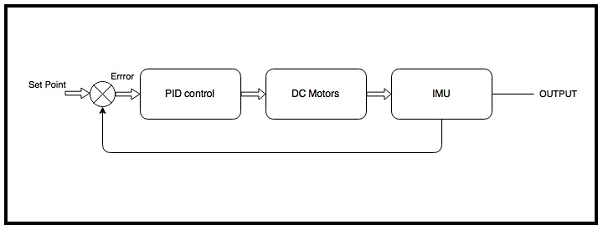
\includegraphics[scale=0.6]{PID.png}
    \end{figure} \\
    \textbf{Set point} is the filtered angle at which bot is balanced which is zero degree in our case.\textbf{Error} is the difference between current angle of the bot and Set point.This is the input to the PID controller.The task of PID controller is to minimise this error close to zero and maintaing Set point in order to balance the bot.\\
    Now question is what happens within PID controller? How did it calculate the output? \\
    The error gets managed in three ways within PID controller.the error is used to execute the propotional term,integral term and derivative term.The mathematical equation for PID is given as:-
    \begin{quote}
    	\centering $ u(t) = Kp*e(t) + Ki* \int_{0}^{t}e(t)\,dt\ + Kd*\frac{de(t)}{dt} $
    \end{quote}
     The Kp, Ki, and Kd are referred as the
     proportional, integral, and derivative constants (the three terms get multiplied by these constants respectively).
     
     To implement this equation we introduced sample time  $\Delta t$ at which PID is calculating the output,so above equation can be written as:-
      \begin{quote}
      	\centering  $ u(t) = Kp*e(t) + Ki*e(t)*\Delta t +Kd*\frac{(e_new - e_old)}{\Delta t} $
      \end{quote}
    As $\Delta t$ is a constant so,
     \begin{quote}
     	\centering  $u(t) = kp*e(t) + ki*e(t) + kd*(e_{new} - e_{old})$
     \end{quote}
    Where kp = Kp \\
          ki = $Ki*\Delta t$  \\
          kd = $\frac{Kd}{\Delta t}$ \\ \\
          
    The PID control algorithm can be modelled in mathematical presentation as:- \\
    \textbf{Output} = Kp*error + Ki*Iterm + Kd* (currenterror-lasterror);\\
   
    The \textbf{proportional} term is obvious as it should be directly proportional to the error.The \textbf{integral} term is sum of all the previous errors.The \textbf{derivative} term is the difference between current error and previous error.\\
    \textbf{Signficance of each term:-}\\
    \textbf{Proportional:-}If only the proportional term had been used to calculate the output, the robot would have reacted in the same way as in the classical line following algorithm.It forces output to reach as close as setpoint but we never reach to the balanced condition.\\
    \textbf{Integral:-} The integral term forces the robot to move towards the mean position or setpoint faster.It decreases response time but we get overshoots in the responses which causes oscillations of the bot .Too much integral term  makes the bot unstable.\\
    \textbf{Derivative:-}The derivative term resists sudden changes in deviation.It reduces the oscillations caused by integral term.\\ \\
     \\ \\ \\ \\ \\ \\ \\ \\ \\ \\ \\ \\
    Following is the code for PID controller:-
    \begin{figure}[h]
    	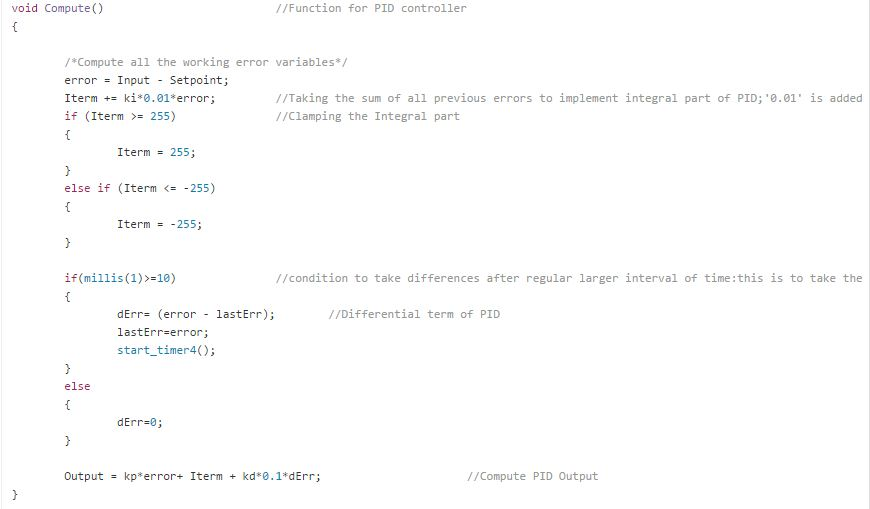
\includegraphics[scale=0.6]{PID_CODE.jpg}
    \end{figure} \\
    As you can see above error is input to pid controller,which is difference between input(current angle of the bot) and setpoint.Iterm is integral term of PID,we are taking sum of all previous errors.We clamped Iterm to 255 to prevent it to become more and more as it can make the response worst.We multiplied it to 0.01 just to be more precise to do fine tuning upto two decimal values of ki.dErr is the derivative term of PID.We are calculating or sampling derivative term after each 10milisecond to make the effect of derivative term more on the response of the bot.If sampled time is too less then derivative term is too smal to make any impact to the system performance. \\ \\
    \textbf{PID tuning:-} \\
    The major challenge for us was to get the proper values of the parameters kp,ki and kd of the PID.Frankly speaking it was very frustrating to tune PID as there is no any proper method available to tune PID.We had to do it by exparimentally.\\
    Here are some steps which will help to get Kp, Ki and Kd faster :\\
    \begin{itemize}
    	\item First set ki and kd to zero and adjust kp so that the robot starts to move about the balance position. P should be large enough for the robot to move but not too large otherwise the movement would not be smooth.
    	\item With kp set, increase ki so that the robot accelerates faster when off balance. It may cause oscillations because of overshoots.Dont increase ki too much otherwise more oscillations makes the response worst. With kp and ki properly tuned, the robot should be able to self-balance for at least a few seconds.
    	\item Finally, increase kd so that the robot would move about its balanced position more gentle, and there shouldn’t be any significant overshoots.
    	\item It is good practice first increase kp,ki and kd in integers,after getting some rough values go for first decimal values around that,then go upto second decimal values and so on.This helps in fine tuning of PID controller.
    \end{itemize} 
    Following is the function for setting tuning parameters :-
    \begin{figure}[h]
    	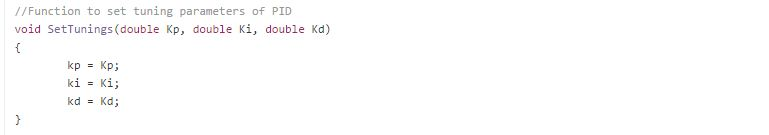
\includegraphics{tuning.jpg}
    \end{figure} \\
    
    After the PID algorithm processes the error, the controller produces a output control signal u. The PID control signal then gets fed into the process under control.In our bot PID controls the speed of motors to get the setpoint at the output.\\ \\ \\ \\ \\ \\ \\ \\ \\ \\ \\ \\ 
    Following is the code for mapping PID output to the speed of the motors:-
    \begin{figure}
    	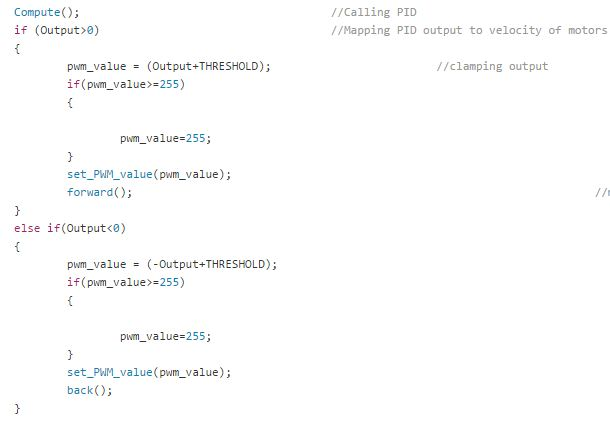
\includegraphics[scale=0.7]{mapping.jpg}
    \end{figure}
    When PID output is positive,means bot is falling in forward direction.We set the pwm values for motors as output+THRESHOLD,where threshold is the minimum pwm value at which motor just starts to rotate.As we are using 8-bit PWM so we clamped pwm values to 255.So to prevent the bot from falling bot will move in forward direction until it will reach to the setpoint.Similarly for backward direction also.\\
    \textbf{Motion of the bot:-} \\
    After the fine tuning, bot was able to balance without any extra support.Now think how it will move forward and backward?...it is very simple...think...think!! \\ \\
  I think you are getting it right.We introduced error into the PID controller intentionally or manually by changing the set point of the bot.Error is positive in forward direction and negative in backward direction.Now PID will try to compensate this error consequently bot will move in forward direction if error is positive and viceversa.
     
    
\end{document}